\section{Auswertung}
\label{sec:Auswertung}

Zunächst soll der Selektivverstärker untersucht werden. Dabei wurden folgende Messwerte aufgenommen:

\begin{table}[H]
  \centering
  \caption{Messwerte des Selektivverstärkers}
  \label{tab:mag}
  \begin{tabular}{c c}
   \toprule
    Frequenz [kHz] & Spannung [mV]\\
   \midrule
   32 & 20.5 \\
   36 & 21.7 \\
   37 & 22.1 \\
   45 & 23.8 \\
   49 & 24.8 \\
   58 & 25.9 \\
   66 & 27.1 \\
  110 & 30.3 \\
  145 & 31.3 \\
  250 & 33   \\
  320 & 33.7 \\
  400 & 34   \\
  450 & 34.3 \\
  1500 & 35.2 \\
  1800 & 35.3 \\
  1950 & 35.7 \\
  1900 & 35.8 \\
  1500 & 35.9 \\
  1200 & 36   \\
  800 & 36.4 \\
  290 & 37.6 \\
  220 & 39.5 \\
  150 & 39.9 \\
  120 & 41.1 \\
  100 & 42.1 \\
   \bottomrule
  \end{tabular}
 \end{table} 

\begin{figure}[H]
  \centering
  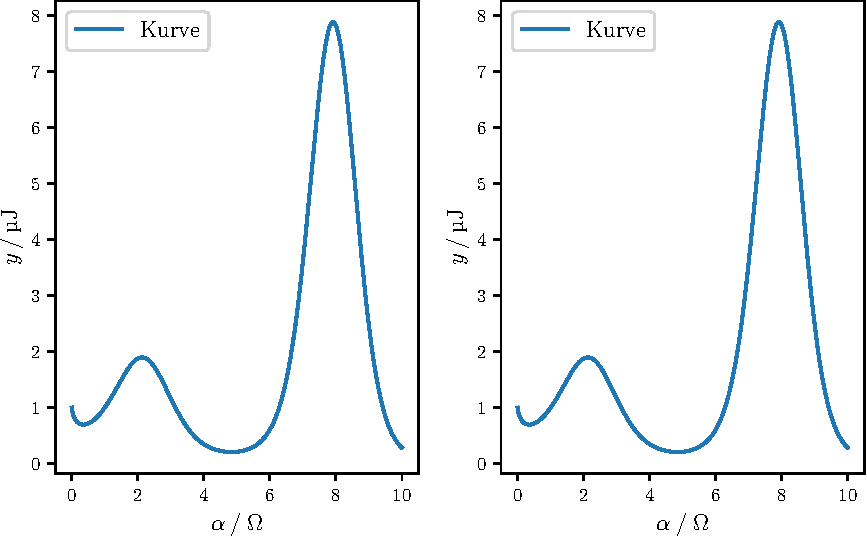
\includegraphics{build/plot.pdf}
  \caption{Filterkurve des Selektivverstärkers.}
  \label{fig:plot}
\end{figure}

Diese Werte sind in Abbildung \ref{fig:plot} dargestellt und durch einen Fit der Form
$ y = e^{-b \cdot (x-a)^{2}}$ angenähert. Es ergeben sich die folgenden Parameter:
\begin{align*}
  a=35460.3 \pm 47.6 \\
  b=(1.01\pm0.13)\cdot 10^{-6}
\end{align*}
Somit kann die Güte zu
\begin{equation*}
  Q=12.78\pm 2.8
\end{equation*}
bestimmt werden. Die Unsicherheiten wurden mittels unumpy berechnet.

\subsection{Bestimmung der Suszeptibilitäten}

\begin{table}[H]
  \centering
  \caption{Messwerte für Gd$_2$O$_3$}
  \label{tab:mag1}
  \begin{tabular}{c c c c}
   \toprule
    $U_0$ [V] & $R_0 [\si{\ohm}]$ &  $U_m$ [V] & $R_m [\si{\ohm}]$ \\
   \midrule
    0.0034 & 2.25 & 0.005  & 1.25  \\
    0.0034 & 2.25 & 0.0047 & 1.225 \\
    0.0034 & 2.06 & 0.0044 & 1.255 \\
   \bottomrule
  \end{tabular}
 \end{table} 

 \begin{table}[H]
  \centering
  \caption{Messwerte für Dy$_2$O$_3$}
  \label{tab:mag2}
  \begin{tabular}{c c c c}
   \toprule
    $U_0$ [V] & $R_0 [\si{\ohm}]$ &  $U_m$ [V] & $R_m [\si{\ohm}]$ \\
   \midrule
    0.0034 & 2.325 & 0.425 & 0.0028 \\
    0.0034 & 2.16  & 0.5   & 0.0028 \\
    0.0034 & 2.12  & 0.48  & 0.0028 \\
    \bottomrule
   \end{tabular}
  \end{table} 
 In den Tabellen steht $U_O$ für das Minimum der Brückenspannung und $R_0$ für den zugehörigen 
 Widerstand ohne Spule. $U_m$ dagegen ist die Spannung, sobald eine Probe eingeführt
 wird und $R_m$ den zum Minimum der Spannung anliegenden Widerstand.
 Aus den Mittelwerten der Messwerte und unter Verwendung der verschiedenen Methoden zur
 Berechnung der Suszeptibilität ergeben sich die folgenden Suszeptibilitäten:
 \begin{table}[H]
  \centering
  \caption{Suszeptibilitäten}
  \label{tab:mag}
  \begin{tabular}{c c c c}
   \toprule
    & $\chi_U$ & $\chi_R$ & $\chi_{theo}$\\
   \midrule
    Gd$_2$O$_3$ & 0.0032 & 0.015 \pm 0.005  & 0.0069\\
    Dy$_2$O$_3$ & 0.0035 & 0.034 \pm 0.0035 & 0.0126\\
   \bottomrule
  \end{tabular}
 \end{table} 

Aufgrund der sehr geringen Abweichungen bei den durch die Spannung bestimmten Suszeptibilitäten
wurden diese nicht aufgeführt. Die theoretischen Werte für die Suszeptibilität konnten aus den 
in Tabelle aufgelisteten Eigenschaften der verwendeten Materialien durch die in der Theorie 
hergeleitete Methode gewonnen werden.

\begin{table}[H]
  \centering
  \caption{Werte der Proben.}
  \label{tab:Proben}
  \begin{tabular}{c c c c c c }
    \toprule
    {Stoff} & {$\rho$ [$\si{\gram\per\centi\metre\cubed}$]} & {$m$ [$\si{\gram}$]} & {$l$ [$\si{\centi\metre}$]} & {$M$ [$\si{\gram\per\mole}$]} & {$Q$ [$\si{\centi\metre\squared}$]}\\
    \midrule
    $\ce{Dy2O3}$ & 7.8 & 15.1 & 17.3 & 372.9982 & 0.1119\\
    $\ce{Gd2O3}$ & 7.4 & 14.08 & 17.5 & 362.4982 & 0.1087\\
    \bottomrule
  \end{tabular}
\end{table}

\begin{table}[H]
  \centering
  \caption{Quantenzahlen und Landé-Faktoren.}
  \begin{tabular}{c c c c c }
    \toprule
    {Stoff} & {$L$} & {$S$} & {$J$} & {$g_J$}\\
    \midrule
    $\ce{Dy2O3}$ & 5 & 2.5 & 7.5 & 1.33\\
    $\ce{Gd2O3}$ & 0 & 3.5 & 3.5 & 2.0\\
    \bottomrule
  \end{tabular}
\end{table}

